\documentclass{article}\usepackage[]{graphicx}\usepackage[]{color}
% maxwidth is the original width if it is less than linewidth
% otherwise use linewidth (to make sure the graphics do not exceed the margin)
\makeatletter
\def\maxwidth{ %
  \ifdim\Gin@nat@width>\linewidth
    \linewidth
  \else
    \Gin@nat@width
  \fi
}
\makeatother

\definecolor{fgcolor}{rgb}{0.345, 0.345, 0.345}
\newcommand{\hlnum}[1]{\textcolor[rgb]{0.686,0.059,0.569}{#1}}%
\newcommand{\hlstr}[1]{\textcolor[rgb]{0.192,0.494,0.8}{#1}}%
\newcommand{\hlcom}[1]{\textcolor[rgb]{0.678,0.584,0.686}{\textit{#1}}}%
\newcommand{\hlopt}[1]{\textcolor[rgb]{0,0,0}{#1}}%
\newcommand{\hlstd}[1]{\textcolor[rgb]{0.345,0.345,0.345}{#1}}%
\newcommand{\hlkwa}[1]{\textcolor[rgb]{0.161,0.373,0.58}{\textbf{#1}}}%
\newcommand{\hlkwb}[1]{\textcolor[rgb]{0.69,0.353,0.396}{#1}}%
\newcommand{\hlkwc}[1]{\textcolor[rgb]{0.333,0.667,0.333}{#1}}%
\newcommand{\hlkwd}[1]{\textcolor[rgb]{0.737,0.353,0.396}{\textbf{#1}}}%
\let\hlipl\hlkwb

\usepackage{framed}
\makeatletter
\newenvironment{kframe}{%
 \def\at@end@of@kframe{}%
 \ifinner\ifhmode%
  \def\at@end@of@kframe{\end{minipage}}%
  \begin{minipage}{\columnwidth}%
 \fi\fi%
 \def\FrameCommand##1{\hskip\@totalleftmargin \hskip-\fboxsep
 \colorbox{shadecolor}{##1}\hskip-\fboxsep
     % There is no \\@totalrightmargin, so:
     \hskip-\linewidth \hskip-\@totalleftmargin \hskip\columnwidth}%
 \MakeFramed {\advance\hsize-\width
   \@totalleftmargin\z@ \linewidth\hsize
   \@setminipage}}%
 {\par\unskip\endMakeFramed%
 \at@end@of@kframe}
\makeatother

\definecolor{shadecolor}{rgb}{.97, .97, .97}
\definecolor{messagecolor}{rgb}{0, 0, 0}
\definecolor{warningcolor}{rgb}{1, 0, 1}
\definecolor{errorcolor}{rgb}{1, 0, 0}
\newenvironment{knitrout}{}{} % an empty environment to be redefined in TeX

\usepackage{alltt}
\usepackage[margin=1in]{geometry}
\IfFileExists{upquote.sty}{\usepackage{upquote}}{}
\begin{document}
\begin{knitrout}
\definecolor{shadecolor}{rgb}{0.969, 0.969, 0.969}\color{fgcolor}\begin{kframe}
\begin{alltt}
\hlcom{# set working directory}
\hlkwd{setwd}\hlstd{(}\hlstr{"C:/Users/jaosi/Desktop/DS-Projects/graduate-project/prostate-cancer"}\hlstd{)}

\hlcom{# load dataset}
\hlstd{APPENC05} \hlkwb{<-} \hlkwd{read.csv}\hlstd{(}\hlstr{"./data/processed/APPENC05.txt"}\hlstd{)}
\hlstd{mydata} \hlkwb{<-} \hlstd{APPENC05}
\hlkwd{summary}\hlstd{(mydata)}
\end{alltt}
\begin{verbatim}
##       Obs     Y_HighGradeCancer    PSALevel          CancerVol       
##  Min.   : 1   Min.   :0.0000    Min.   :-2.53370   Min.   :-2.30258  
##  1st Qu.:25   1st Qu.:0.0000    1st Qu.:-0.65227   1st Qu.:-0.71613  
##  Median :49   Median :0.0000    Median : 0.09702   Median : 0.08555  
##  Mean   :49   Mean   :0.2165    Mean   : 0.00000   Mean   : 0.00000  
##  3rd Qu.:73   3rd Qu.:0.0000    3rd Qu.: 0.50654   3rd Qu.: 0.66550  
##  Max.   :97   Max.   :1.0000    Max.   : 2.70223   Max.   : 2.10683  
##      Weight             Age          BenignProstaticHyperplasia
##  Min.   :-2.5953   Min.   :-3.0872   Min.   :-0.8406           
##  1st Qu.:-0.5519   1st Qu.:-0.5220   1st Qu.:-0.8406           
##  Median :-0.0663   Median : 0.1531   Median :-0.3929           
##  Mean   : 0.0000   Mean   : 0.0000   Mean   : 0.0000           
##  3rd Qu.: 0.4597   3rd Qu.: 0.5582   3rd Qu.: 0.7375           
##  Max.   : 4.9712   Max.   : 2.0433   Max.   : 2.5678           
##  SeminalVesicleInvasion CapsularPenetration
##  Min.   :0.0000         Min.   :-0.5966    
##  1st Qu.:0.0000         1st Qu.:-0.5966    
##  Median :0.0000         Median :-0.4772    
##  Mean   :0.2165         Mean   : 0.0000    
##  3rd Qu.:0.0000         3rd Qu.: 0.2681    
##  Max.   :1.0000         Max.   : 4.2321
\end{verbatim}
\begin{alltt}
\hlkwd{View}\hlstd{(mydata)}
\hlkwd{names}\hlstd{(mydata)}
\end{alltt}
\begin{verbatim}
## [1] "Obs"                        "Y_HighGradeCancer"         
## [3] "PSALevel"                   "CancerVol"                 
## [5] "Weight"                     "Age"                       
## [7] "BenignProstaticHyperplasia" "SeminalVesicleInvasion"    
## [9] "CapsularPenetration"
\end{verbatim}
\begin{alltt}
\hlcom{# load packages}
\hlkwd{library}\hlstd{(caTools)}
\hlkwd{library}\hlstd{(ROCR)}
\hlkwd{library}\hlstd{(ResourceSelection)}
\end{alltt}


{\ttfamily\noindent\color{warningcolor}{\#\# Warning: package 'ResourceSelection' was built under R version 4.0.3}}

{\ttfamily\noindent\itshape\color{messagecolor}{\#\# ResourceSelection 0.3-5 	 2019-07-22}}\begin{alltt}
\hlkwd{library}\hlstd{(car)}
\end{alltt}


{\ttfamily\noindent\color{warningcolor}{\#\# Warning: package 'car' was built under R version 4.0.3}}

{\ttfamily\noindent\itshape\color{messagecolor}{\#\# Loading required package: carData}}

{\ttfamily\noindent\color{warningcolor}{\#\# Warning: package 'carData' was built under R version 4.0.3}}\begin{alltt}
\hlcom{# declare SeminalVesicleInvasion a categorical variable (SeminalVesicleInvasion == [0, 1])}
\hlstd{mydata}\hlopt{$}\hlstd{SeminalVesicleInvasion} \hlkwb{<-} \hlkwd{factor}\hlstd{(mydata}\hlopt{$}\hlstd{SeminalVesicleInvasion)}

\hlcom{# create training and testing subsets}
\hlstd{myseed} \hlkwb{<-} \hlnum{123}
\hlkwd{set.seed}\hlstd{(myseed)}
\hlstd{split} \hlkwb{<-} \hlkwd{sample.split}\hlstd{(mydata,} \hlkwc{SplitRatio}\hlstd{=}\hlnum{0.8}\hlstd{)}
\hlstd{train} \hlkwb{<-} \hlkwd{subset}\hlstd{(mydata, split}\hlopt{==}\hlstr{"TRUE"}\hlstd{)}
\hlstd{test} \hlkwb{<-} \hlkwd{subset}\hlstd{(mydata, split}\hlopt{==}\hlstr{"FALSE"}\hlstd{)}

\hlkwd{View}\hlstd{(train)}
\hlkwd{View}\hlstd{(test)}

\hlcom{# write train & test datasets to CSV files}
\hlkwd{write.csv}\hlstd{(train,} \hlstr{"./data/processed/train.txt"}\hlstd{)}
\hlkwd{write.csv}\hlstd{(test,} \hlstr{"./data/processed/test.txt"}\hlstd{)}


\hlcom{##################################}
\hlcom{### Building Helpful Functions ###}
\hlcom{##################################}

\hlstd{freq} \hlkwb{<-} \hlkwa{function}\hlstd{(}\hlkwc{data}\hlstd{) \{}
  \hlcom{### function requires one input parameter: data.}
  \hlcom{### this function will display the table of Y_HighGradeCancer counts (frequency table);}
  \hlcom{# i.e. the counts of 0's and 1's in the input data.}
  \hlcom{### the function will then display the proportion of 0 to 1 (I already know via}
  \hlcom{# previous analysis that the counts of 0's greatly outweigh the count of 1's).}
  \hlcom{### we can consider this proportion to be a "base accuracy" for model comparison;}
  \hlcom{# i.e. if the model just predicted 0's (most frequent classification),}
  \hlcom{# for all cases.}

  \hlstd{name} \hlkwb{<-} \hlkwd{deparse}\hlstd{(}\hlkwd{substitute}\hlstd{(data))}

  \hlkwa{if} \hlstd{(name}\hlopt{==}\hlstr{'train'}\hlstd{) \{}
    \hlkwd{cat}\hlstd{(}\hlstr{'TRAINING DATA\textbackslash{}n'}\hlstd{)}
  \hlstd{\}}
  \hlkwa{else} \hlstd{\{}
    \hlkwd{cat}\hlstd{(}\hlstr{'TESTING DATA\textbackslash{}n'}\hlstd{)}
  \hlstd{\}}

  \hlstd{freq_tab} \hlkwb{<-} \hlkwd{table}\hlstd{(data}\hlopt{$}\hlstd{Y_HighGradeCancer)}
  \hlstd{most_freq_prop} \hlkwb{<-} \hlkwd{round}\hlstd{(}\hlkwd{sum}\hlstd{(freq_tab[}\hlnum{1}\hlstd{])}\hlopt{/}\hlkwd{sum}\hlstd{(freq_tab),} \hlnum{4}\hlstd{)}
  \hlstd{less_freq_pop} \hlkwb{<-} \hlkwd{round}\hlstd{(}\hlkwd{sum}\hlstd{(freq_tab[}\hlnum{2}\hlstd{])}\hlopt{/}\hlkwd{sum}\hlstd{(freq_tab),} \hlnum{4}\hlstd{)}

  \hlcom{# print out both the table, and calculated base accuracy }
  \hlkwd{cat}\hlstd{(}\hlstr{'Frequency Table:\textbackslash{}n'}\hlstd{)}
  \hlkwd{print}\hlstd{(freq_tab)}
  \hlkwd{cat}\hlstd{(}\hlstr{'\textbackslash{}nThe proportion of 0 to 1 is:'}\hlstd{, most_freq_prop,} \hlstr{'\textbackslash{}n'}\hlstd{)}
  \hlkwd{cat}\hlstd{(}\hlstr{'The proportion of 1 to 0 is:'}\hlstd{, less_freq_pop)}
\hlstd{\}}


\hlstd{accuracy} \hlkwb{<-} \hlkwa{function}\hlstd{(}\hlkwc{model}\hlstd{,} \hlkwc{data}\hlstd{,} \hlkwc{val}\hlstd{=}\hlnum{0.50}\hlstd{) \{}
  \hlcom{### function requires three input parameters: model, data, and decision value boundry}
  \hlcom{# (optional); defualt 50%.}
  \hlcom{### this function will first apply the fitted model and create classifications,}
  \hlcom{# then compare to real values (which we know).}
  \hlcom{### the confusion matrix and accuracy score will output to the terminal.}
  \hlcom{### idealy we want the accuracy score to be greater than the base score calculated}
  \hlcom{# previously (this indicates the logistic model is a better fit).}
  \hlcom{### decision boundry value may require analysis and adjustments/optimizations afterwards.}

  \hlstd{name} \hlkwb{<-} \hlkwd{deparse}\hlstd{(}\hlkwd{substitute}\hlstd{(data))}

  \hlkwa{if} \hlstd{(name}\hlopt{==}\hlstr{'train'}\hlstd{) \{}
    \hlkwd{cat}\hlstd{(}\hlstr{'TRAINING DATA\textbackslash{}n'}\hlstd{)}
  \hlstd{\}}
  \hlkwa{else} \hlstd{\{}
    \hlkwd{cat}\hlstd{(}\hlstr{'TESTING DATA\textbackslash{}n'}\hlstd{)}
  \hlstd{\}}

  \hlstd{res} \hlkwb{<-} \hlkwd{predict}\hlstd{(model, data,} \hlkwc{type}\hlstd{=}\hlstr{"response"}\hlstd{)}
  \hlstd{tab} \hlkwb{<-} \hlkwd{table}\hlstd{(}\hlkwc{ActualValue}\hlstd{=data}\hlopt{$}\hlstd{Y_HighGradeCancer,} \hlkwc{PredictedValue}\hlstd{=res}\hlopt{>=}\hlstd{val)}
  \hlstd{err} \hlkwb{<-} \hlkwd{round}\hlstd{((}\hlnum{1}\hlopt{-}\hlstd{(}\hlkwd{sum}\hlstd{(}\hlkwd{diag}\hlstd{(tab))}\hlopt{/}\hlkwd{sum}\hlstd{(tab)))}\hlopt{*}\hlnum{100}\hlstd{,} \hlnum{1}\hlstd{)}
  \hlstd{acc} \hlkwb{<-} \hlkwd{round}\hlstd{(}\hlkwd{sum}\hlstd{(}\hlkwd{diag}\hlstd{(tab))}\hlopt{/}\hlkwd{sum}\hlstd{(tab)}\hlopt{*}\hlnum{100}\hlstd{,} \hlnum{1}\hlstd{)}

  \hlcom{# print out confusion matrix, and calculated accuracy}
  \hlkwd{cat}\hlstd{(}\hlstr{'Prediction Rule:'}\hlstd{, val,} \hlstr{'\textbackslash{}n'}\hlstd{)}
  \hlkwd{cat}\hlstd{(}\hlstr{'Confusion Matrix:\textbackslash{}n'}\hlstd{,} \hlstr{'\textbackslash{}n'}\hlstd{)}
  \hlkwd{print}\hlstd{(tab)}
  \hlkwd{cat}\hlstd{(}\hlstr{'\textbackslash{}nThe calculated error is:'}\hlstd{, err,} \hlstr{'%'}\hlstd{)}
  \hlkwd{cat}\hlstd{(}\hlstr{'\textbackslash{}nThe calculated accuracy is:'}\hlstd{, acc,} \hlstr{'%'}\hlstd{)}
\hlstd{\}}



\hlcom{##########################}
\hlcom{###                    ###}
\hlcom{###    Model Fitting   ###}
\hlcom{###                    ###}
\hlcom{##########################}

\hlcom{###############################################}
\hlcom{### Second-Order Polynomial Logistic Models ###}
\hlcom{###############################################}

\hlcom{# fit full second-order logistic model}
\hlstd{logit_poly} \hlkwb{<-} \hlkwd{glm}\hlstd{(Y_HighGradeCancer} \hlopt{~} \hlkwd{poly}\hlstd{(PSALevel,} \hlnum{2}\hlstd{)} \hlopt{+} \hlkwd{poly}\hlstd{(CancerVol,} \hlnum{2}\hlstd{)} \hlopt{+}
                    \hlkwd{poly}\hlstd{(Weight,} \hlnum{2}\hlstd{)} \hlopt{+} \hlkwd{poly}\hlstd{(Age,} \hlnum{2}\hlstd{)} \hlopt{+} \hlkwd{poly}\hlstd{(BenignProstaticHyperplasia,} \hlnum{2}\hlstd{)} \hlopt{+}
                    \hlstd{SeminalVesicleInvasion} \hlopt{+} \hlkwd{poly}\hlstd{(CapsularPenetration,} \hlnum{2}\hlstd{),}
                  \hlkwc{data}\hlstd{=train,} \hlkwc{family}\hlstd{=}\hlstr{"binomial"}\hlstd{)}
\hlkwd{summary}\hlstd{(logit_poly)}
\end{alltt}
\begin{verbatim}
## 
## Call:
## glm(formula = Y_HighGradeCancer ~ poly(PSALevel, 2) + poly(CancerVol, 
##     2) + poly(Weight, 2) + poly(Age, 2) + poly(BenignProstaticHyperplasia, 
##     2) + SeminalVesicleInvasion + poly(CapsularPenetration, 2), 
##     family = "binomial", data = train)
## 
## Deviance Residuals: 
##      Min        1Q    Median        3Q       Max  
## -1.56947  -0.29292  -0.11807  -0.02792   2.70547  
## 
## Coefficients:
##                                      Estimate Std. Error z value Pr(>|z|)   
## (Intercept)                           -3.1879     1.1911  -2.676  0.00744 **
## poly(PSALevel, 2)1                     8.8748     9.4300   0.941  0.34664   
## poly(PSALevel, 2)2                     9.9300     9.7971   1.014  0.31079   
## poly(CancerVol, 2)1                    9.0626    12.3092   0.736  0.46158   
## poly(CancerVol, 2)2                    3.7797     8.9295   0.423  0.67209   
## poly(Weight, 2)1                      -1.7984     8.8561  -0.203  0.83908   
## poly(Weight, 2)2                     -22.1802    19.1499  -1.158  0.24676   
## poly(Age, 2)1                          3.0558     5.5976   0.546  0.58513   
## poly(Age, 2)2                          6.6241     4.6130   1.436  0.15102   
## poly(BenignProstaticHyperplasia, 2)1   8.0033     7.2503   1.104  0.26966   
## poly(BenignProstaticHyperplasia, 2)2   6.8035     6.3958   1.064  0.28745   
## SeminalVesicleInvasion1               -0.9176     1.1728  -0.782  0.43397   
## poly(CapsularPenetration, 2)1          2.4574     3.9676   0.619  0.53568   
## poly(CapsularPenetration, 2)2         -7.9544     4.4302  -1.795  0.07258 . 
## ---
## Signif. codes:  0 '***' 0.001 '**' 0.01 '*' 0.05 '.' 0.1 ' ' 1
## 
## (Dispersion parameter for binomial family taken to be 1)
## 
##     Null deviance: 72.613  on 75  degrees of freedom
## Residual deviance: 33.998  on 62  degrees of freedom
## AIC: 61.998
## 
## Number of Fisher Scoring iterations: 8
\end{verbatim}
\begin{alltt}
\hlkwd{step}\hlstd{(logit_poly,} \hlkwc{direction}\hlstd{=}\hlstr{"backward"}\hlstd{)}
\end{alltt}
\begin{verbatim}
## Start:  AIC=62
## Y_HighGradeCancer ~ poly(PSALevel, 2) + poly(CancerVol, 2) + 
##     poly(Weight, 2) + poly(Age, 2) + poly(BenignProstaticHyperplasia, 
##     2) + SeminalVesicleInvasion + poly(CapsularPenetration, 2)
## 
##                                       Df Deviance    AIC
## - poly(CancerVol, 2)                   2   35.756 59.756
## - poly(BenignProstaticHyperplasia, 2)  2   35.913 59.913
## - SeminalVesicleInvasion               1   34.644 60.644
## - poly(Weight, 2)                      2   36.698 60.698
## <none>                                     33.998 61.998
## - poly(CapsularPenetration, 2)         2   38.078 62.078
## - poly(Age, 2)                         2   38.511 62.511
## - poly(PSALevel, 2)                    2   40.072 64.072
## 
## Step:  AIC=59.76
## Y_HighGradeCancer ~ poly(PSALevel, 2) + poly(Weight, 2) + poly(Age, 
##     2) + poly(BenignProstaticHyperplasia, 2) + SeminalVesicleInvasion + 
##     poly(CapsularPenetration, 2)
## 
##                                       Df Deviance    AIC
## - poly(BenignProstaticHyperplasia, 2)  2   37.400 57.400
## - poly(Weight, 2)                      2   38.191 58.191
## - SeminalVesicleInvasion               1   36.552 58.552
## <none>                                     35.756 59.756
## - poly(Age, 2)                         2   39.906 59.906
## - poly(CapsularPenetration, 2)         2   42.124 62.124
## - poly(PSALevel, 2)                    2   47.961 67.961
## 
## Step:  AIC=57.4
## Y_HighGradeCancer ~ poly(PSALevel, 2) + poly(Weight, 2) + poly(Age, 
##     2) + SeminalVesicleInvasion + poly(CapsularPenetration, 2)
## 
##                                Df Deviance    AIC
## - poly(Weight, 2)               2   38.338 54.338
## - SeminalVesicleInvasion        1   38.128 56.128
## <none>                              37.400 57.400
## - poly(Age, 2)                  2   43.065 59.065
## - poly(CapsularPenetration, 2)  2   43.734 59.734
## - poly(PSALevel, 2)             2   48.695 64.695
## 
## Step:  AIC=54.34
## Y_HighGradeCancer ~ poly(PSALevel, 2) + poly(Age, 2) + SeminalVesicleInvasion + 
##     poly(CapsularPenetration, 2)
## 
##                                Df Deviance    AIC
## - SeminalVesicleInvasion        1   38.900 52.900
## <none>                              38.338 54.338
## - poly(Age, 2)                  2   44.099 56.099
## - poly(CapsularPenetration, 2)  2   46.605 58.605
## - poly(PSALevel, 2)             2   51.230 63.230
## 
## Step:  AIC=52.9
## Y_HighGradeCancer ~ poly(PSALevel, 2) + poly(Age, 2) + poly(CapsularPenetration, 
##     2)
## 
##                                Df Deviance    AIC
## <none>                              38.900 52.900
## - poly(Age, 2)                  2   44.200 54.200
## - poly(CapsularPenetration, 2)  2   46.739 56.739
## - poly(PSALevel, 2)             2   51.888 61.888
## 
## Call:  glm(formula = Y_HighGradeCancer ~ poly(PSALevel, 2) + poly(Age, 
##     2) + poly(CapsularPenetration, 2), family = "binomial", data = train)
## 
## Coefficients:
##                   (Intercept)             poly(PSALevel, 2)1  
##                        -2.604                         12.807  
##            poly(PSALevel, 2)2                  poly(Age, 2)1  
##                         7.005                          2.768  
##                 poly(Age, 2)2  poly(CapsularPenetration, 2)1  
##                         6.363                          4.741  
## poly(CapsularPenetration, 2)2  
##                        -8.417  
## 
## Degrees of Freedom: 75 Total (i.e. Null);  69 Residual
## Null Deviance:	    72.61 
## Residual Deviance: 38.9 	AIC: 52.9
\end{verbatim}
\begin{alltt}
\hlcom{# use second-order reduced model setup for quick analysis of adding/removing predictors}
\hlstd{logit_poly_red} \hlkwb{<-} \hlkwd{glm}\hlstd{(Y_HighGradeCancer} \hlopt{~}
                        \hlkwd{poly}\hlstd{(PSALevel,} \hlnum{2}\hlstd{)}
                      \hlopt{+} \hlkwd{poly}\hlstd{(CancerVol,} \hlnum{2}\hlstd{)}
                      \hlcom{# + poly(Weight, 2) }
                      \hlcom{# + poly(Age, 2)}
                      \hlcom{# + poly(BenignProstaticHyperplasia, 2)}
                      \hlcom{# + poly(SeminalVesicleInvasion, 2) }
                      \hlcom{#  + poly(CapsularPenetration, 2)}
                      \hlstd{,} \hlkwc{data}\hlstd{=train,} \hlkwc{family}\hlstd{=}\hlstr{"binomial"}\hlstd{)}
\hlkwd{summary}\hlstd{(logit_poly_red)}
\end{alltt}
\begin{verbatim}
## 
## Call:
## glm(formula = Y_HighGradeCancer ~ poly(PSALevel, 2) + poly(CancerVol, 
##     2), family = "binomial", data = train)
## 
## Deviance Residuals: 
##      Min        1Q    Median        3Q       Max  
## -1.65643  -0.46122  -0.20861  -0.01794   2.41869  
## 
## Coefficients:
##                     Estimate Std. Error z value Pr(>|z|)  
## (Intercept)          -2.9802     1.2771  -2.334   0.0196 *
## poly(PSALevel, 2)1    9.0035     8.1120   1.110   0.2670  
## poly(PSALevel, 2)2    0.6259     7.4678   0.084   0.9332  
## poly(CancerVol, 2)1  17.9731    14.8783   1.208   0.2270  
## poly(CancerVol, 2)2  -3.3028    10.0734  -0.328   0.7430  
## ---
## Signif. codes:  0 '***' 0.001 '**' 0.01 '*' 0.05 '.' 0.1 ' ' 1
## 
## (Dispersion parameter for binomial family taken to be 1)
## 
##     Null deviance: 72.613  on 75  degrees of freedom
## Residual deviance: 44.511  on 71  degrees of freedom
## AIC: 54.511
## 
## Number of Fisher Scoring iterations: 8
\end{verbatim}
\begin{alltt}
\hlkwd{step}\hlstd{(logit_poly_red,} \hlkwc{direction}\hlstd{=}\hlstr{"backward"}\hlstd{)}
\end{alltt}
\begin{verbatim}
## Start:  AIC=54.51
## Y_HighGradeCancer ~ poly(PSALevel, 2) + poly(CancerVol, 2)
## 
##                      Df Deviance    AIC
## - poly(PSALevel, 2)   2   48.120 54.120
## <none>                    44.511 54.511
## - poly(CancerVol, 2)  2   50.767 56.767
## 
## Step:  AIC=54.12
## Y_HighGradeCancer ~ poly(CancerVol, 2)
## 
##                      Df Deviance    AIC
## <none>                    48.120 54.120
## - poly(CancerVol, 2)  2   72.613 74.613
## 
## Call:  glm(formula = Y_HighGradeCancer ~ poly(CancerVol, 2), family = "binomial", 
##     data = train)
## 
## Coefficients:
##         (Intercept)  poly(CancerVol, 2)1  poly(CancerVol, 2)2  
##             -2.6364              20.0802              -0.4743  
## 
## Degrees of Freedom: 75 Total (i.e. Null);  73 Residual
## Null Deviance:	    72.61 
## Residual Deviance: 48.12 	AIC: 54.12
\end{verbatim}
\begin{alltt}
\hlcom{###################################}
\hlcom{### First-Order Logistic Models ###}
\hlcom{###################################}

\hlcom{# fit full first-order logistic model}
\hlstd{logit_full} \hlkwb{<-} \hlkwd{glm}\hlstd{(Y_HighGradeCancer} \hlopt{~} \hlstd{PSALevel} \hlopt{+} \hlstd{CancerVol} \hlopt{+} \hlstd{Weight} \hlopt{+}
                    \hlstd{Age} \hlopt{+} \hlstd{BenignProstaticHyperplasia} \hlopt{+}
                    \hlstd{SeminalVesicleInvasion} \hlopt{+} \hlstd{CapsularPenetration,} \hlkwc{data}\hlstd{=train,}
                  \hlkwc{family}\hlstd{=}\hlstr{"binomial"}\hlstd{)}
\hlkwd{summary}\hlstd{(logit_full)}
\end{alltt}
\begin{verbatim}
## 
## Call:
## glm(formula = Y_HighGradeCancer ~ PSALevel + CancerVol + Weight + 
##     Age + BenignProstaticHyperplasia + SeminalVesicleInvasion + 
##     CapsularPenetration, family = "binomial", data = train)
## 
## Deviance Residuals: 
##      Min        1Q    Median        3Q       Max  
## -1.66861  -0.39211  -0.18721  -0.02467   2.17445  
## 
## Coefficients:
##                            Estimate Std. Error z value Pr(>|z|)    
## (Intercept)                -2.84305    0.75774  -3.752 0.000175 ***
## PSALevel                    1.28155    0.74609   1.718 0.085856 .  
## CancerVol                   1.40464    0.90103   1.559 0.119014    
## Weight                     -0.17618    0.75535  -0.233 0.815567    
## Age                         0.56784    0.43547   1.304 0.192245    
## BenignProstaticHyperplasia  0.07823    0.54237   0.144 0.885320    
## SeminalVesicleInvasion1    -0.38818    1.04075  -0.373 0.709164    
## CapsularPenetration         0.25330    0.44939   0.564 0.572988    
## ---
## Signif. codes:  0 '***' 0.001 '**' 0.01 '*' 0.05 '.' 0.1 ' ' 1
## 
## (Dispersion parameter for binomial family taken to be 1)
## 
##     Null deviance: 72.613  on 75  degrees of freedom
## Residual deviance: 42.303  on 68  degrees of freedom
## AIC: 58.303
## 
## Number of Fisher Scoring iterations: 7
\end{verbatim}
\begin{alltt}
\hlkwd{step}\hlstd{(logit_full,} \hlkwc{direction}\hlstd{=}\hlstr{"backward"}\hlstd{)}
\end{alltt}
\begin{verbatim}
## Start:  AIC=58.3
## Y_HighGradeCancer ~ PSALevel + CancerVol + Weight + Age + BenignProstaticHyperplasia + 
##     SeminalVesicleInvasion + CapsularPenetration
## 
##                              Df Deviance    AIC
## - BenignProstaticHyperplasia  1   42.324 56.324
## - Weight                      1   42.358 56.358
## - SeminalVesicleInvasion      1   42.444 56.444
## - CapsularPenetration         1   42.627 56.627
## - Age                         1   43.954 57.954
## <none>                            42.303 58.303
## - CancerVol                   1   45.225 59.225
## - PSALevel                    1   45.903 59.903
## 
## Step:  AIC=56.32
## Y_HighGradeCancer ~ PSALevel + CancerVol + Weight + Age + SeminalVesicleInvasion + 
##     CapsularPenetration
## 
##                          Df Deviance    AIC
## - Weight                  1   42.358 54.358
## - SeminalVesicleInvasion  1   42.499 54.499
## - CapsularPenetration     1   42.695 54.695
## - Age                     1   44.044 56.044
## <none>                        42.324 56.324
## - CancerVol               1   45.389 57.389
## - PSALevel                1   46.031 58.031
## 
## Step:  AIC=54.36
## Y_HighGradeCancer ~ PSALevel + CancerVol + Age + SeminalVesicleInvasion + 
##     CapsularPenetration
## 
##                          Df Deviance    AIC
## - SeminalVesicleInvasion  1   42.522 52.522
## - CapsularPenetration     1   42.755 52.755
## - Age                     1   44.151 54.151
## <none>                        42.358 54.358
## - CancerVol               1   45.390 55.390
## - PSALevel                1   46.059 56.059
## 
## Step:  AIC=52.52
## Y_HighGradeCancer ~ PSALevel + CancerVol + Age + CapsularPenetration
## 
##                       Df Deviance    AIC
## - CapsularPenetration  1   42.780 50.780
## - Age                  1   44.168 52.168
## <none>                     42.522 52.522
## - CancerVol            1   45.558 53.558
## - PSALevel             1   46.285 54.285
## 
## Step:  AIC=50.78
## Y_HighGradeCancer ~ PSALevel + CancerVol + Age
## 
##             Df Deviance    AIC
## - Age        1   44.628 50.628
## <none>           42.780 50.780
## - PSALevel   1   46.445 52.445
## - CancerVol  1   48.777 54.777
## 
## Step:  AIC=50.63
## Y_HighGradeCancer ~ PSALevel + CancerVol
## 
##             Df Deviance    AIC
## <none>           44.628 50.628
## - PSALevel   1   48.123 52.123
## - CancerVol  1   50.767 54.767
## 
## Call:  glm(formula = Y_HighGradeCancer ~ PSALevel + CancerVol, family = "binomial", 
##     data = train)
## 
## Coefficients:
## (Intercept)     PSALevel    CancerVol  
##      -2.687        1.058        1.550  
## 
## Degrees of Freedom: 75 Total (i.e. Null);  73 Residual
## Null Deviance:	    72.61 
## Residual Deviance: 44.63 	AIC: 50.63
\end{verbatim}
\begin{alltt}
\hlcom{# use reduced model setup for quick analysis of adding/removing predictors}
\hlstd{logit_red} \hlkwb{<-} \hlkwd{glm}\hlstd{(Y_HighGradeCancer} \hlopt{~}
                   \hlstd{PSALevel}
                 \hlopt{+} \hlstd{CancerVol}
                 \hlcom{# + Weight }
                 \hlcom{# + Age}
                 \hlcom{# + BenignProstaticHyperplasia}
                 \hlcom{# + SeminalVesicleInvasion}
                 \hlcom{# + CapsularPenetration}
                 \hlstd{,} \hlkwc{data}\hlstd{=train,} \hlkwc{family}\hlstd{=}\hlstr{"binomial"}\hlstd{)}
\hlkwd{summary}\hlstd{(logit_red)}
\end{alltt}
\begin{verbatim}
## 
## Call:
## glm(formula = Y_HighGradeCancer ~ PSALevel + CancerVol, family = "binomial", 
##     data = train)
## 
## Deviance Residuals: 
##      Min        1Q    Median        3Q       Max  
## -1.73560  -0.43637  -0.23378  -0.03521   2.42555  
## 
## Coefficients:
##             Estimate Std. Error z value Pr(>|z|)    
## (Intercept)  -2.6867     0.6186  -4.343 1.41e-05 ***
## PSALevel      1.0577     0.6198   1.707   0.0879 .  
## CancerVol     1.5502     0.6859   2.260   0.0238 *  
## ---
## Signif. codes:  0 '***' 0.001 '**' 0.01 '*' 0.05 '.' 0.1 ' ' 1
## 
## (Dispersion parameter for binomial family taken to be 1)
## 
##     Null deviance: 72.613  on 75  degrees of freedom
## Residual deviance: 44.628  on 73  degrees of freedom
## AIC: 50.628
## 
## Number of Fisher Scoring iterations: 6
\end{verbatim}
\begin{alltt}
\hlcom{##########################################}
\hlcom{###                                    ###}
\hlcom{###    Model Checking and Validation   ###}
\hlcom{###                                    ###}
\hlcom{##########################################}

\hlcom{################################################################}
\hlcom{### Cook's Distance Diagnostics for Influential Observations ###}
\hlcom{################################################################}
\hlkwd{plot}\hlstd{(logit_red,} \hlkwc{pch}\hlstd{=}\hlnum{18}\hlstd{,} \hlkwc{col}\hlstd{=}\hlstr{"red"}\hlstd{,} \hlkwc{which}\hlstd{=}\hlkwd{c}\hlstd{(}\hlnum{4}\hlstd{))}
\end{alltt}
\end{kframe}
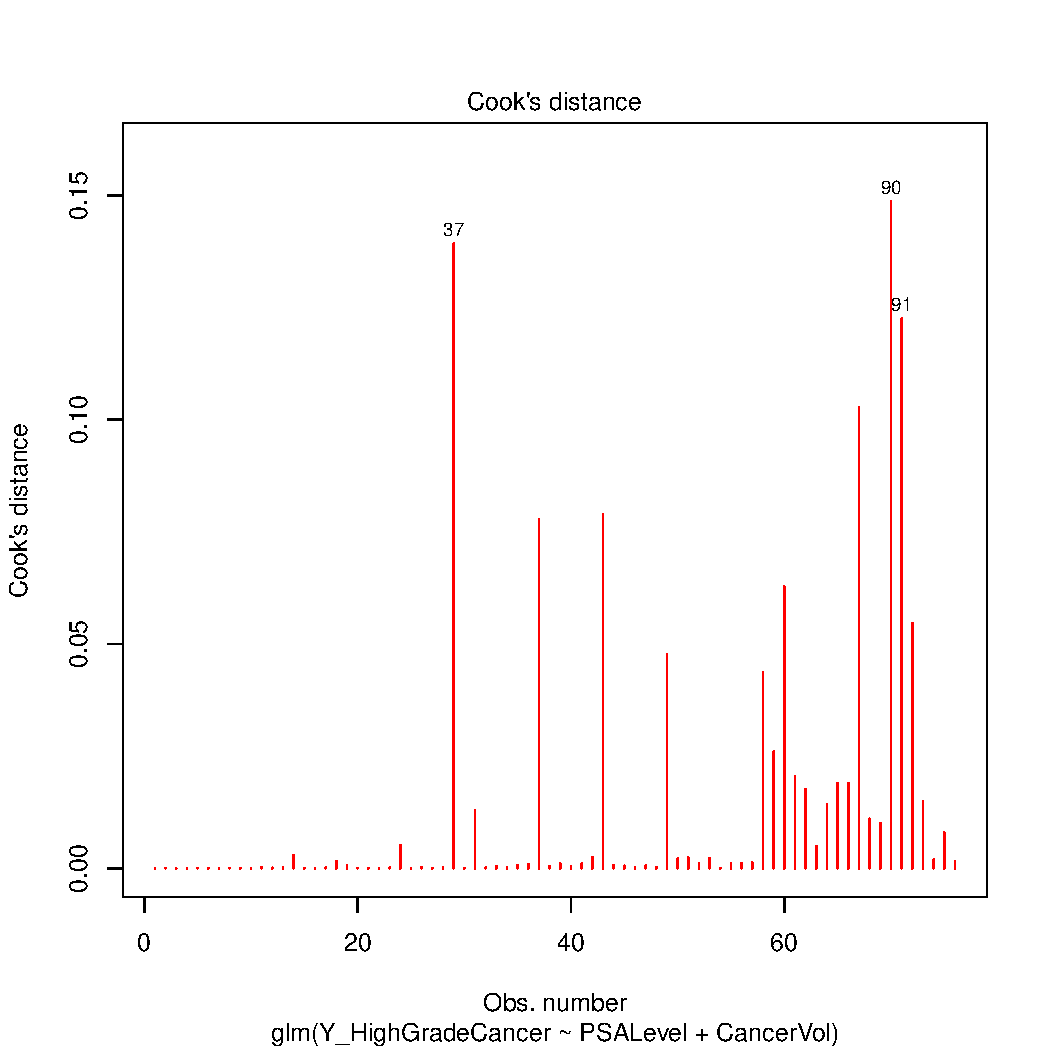
\includegraphics[width=\maxwidth]{figure/unnamed-chunk-1-1} 
\begin{kframe}\begin{alltt}
\hlstd{myCDs} \hlkwb{<-} \hlkwd{sort}\hlstd{(}\hlkwd{round}\hlstd{(}\hlkwd{cooks.distance}\hlstd{(logit_red),} \hlnum{5}\hlstd{),} \hlkwc{decreasing}\hlstd{=}\hlnum{TRUE}\hlstd{)}
\hlstd{myCDs}
\end{alltt}
\begin{verbatim}
##      90      37      91      85      55      47      76      92      63      74 
## 0.14859 0.13928 0.12254 0.10270 0.07886 0.07780 0.06282 0.05464 0.04771 0.04380 
##      75      78      84      83      79      93      82      39      87      88 
## 0.02604 0.02058 0.01905 0.01897 0.01768 0.01504 0.01424 0.01284 0.01107 0.01004 
##      96      30      81      18      54      65      67      64      94      22 
## 0.00797 0.00521 0.00500 0.00290 0.00251 0.00238 0.00224 0.00221 0.00196 0.00158 
##      97      73      72      66      49      70      52      46      24      56 
## 0.00149 0.00131 0.00119 0.00116 0.00110 0.00106 0.00105 0.00092 0.00073 0.00071 
##      45      60      57      42      51      48      13      36      16      61 
## 0.00069 0.00066 0.00057 0.00052 0.00052 0.00048 0.00034 0.00033 0.00032 0.00031 
##      33      58      40      21      29      15      43      38      69      27 
## 0.00029 0.00028 0.00018 0.00015 0.00015 0.00014 0.00014 0.00009 0.00008 0.00005 
##      25      31      34       7      20      10      11      28       1       2 
## 0.00004 0.00004 0.00003 0.00002 0.00002 0.00001 0.00001 0.00001 0.00000 0.00000 
##       3       4       6       9      12      19 
## 0.00000 0.00000 0.00000 0.00000 0.00000 0.00000
\end{verbatim}
\begin{alltt}
\hlcom{# drop rows for model building (influential observations)}
\hlcom{# this step will be visited within Coook's Distance analysis}
\hlstd{train_trim} \hlkwb{<-} \hlkwd{subset}\hlstd{(train, Obs} \hlopt{!=} \hlnum{90}
                     \hlcom{#  & Obs != 37}
                     \hlcom{#  & Obs != 91}
\hlstd{)}

\hlcom{# view the trimmed data}
\hlkwd{View}\hlstd{(train_trim)}

\hlcom{# write train_trim dataset to csv file}
\hlkwd{write.csv}\hlstd{(train_trim,} \hlstr{"./data/processed/train_trim.txt"}\hlstd{)}

\hlcom{# re-fit the logistic model}
\hlstd{logit_red_trim} \hlkwb{<-} \hlkwd{glm}\hlstd{(Y_HighGradeCancer} \hlopt{~}
                        \hlstd{PSALevel}
                      \hlopt{+} \hlstd{CancerVol}
                      \hlcom{# + Weight }
                      \hlcom{# + Age}
                      \hlcom{# + BenignProstaticHyperplasia}
                      \hlcom{# + SeminalVesicleInvasion}
                      \hlcom{# + CapsularPenetration}
                      \hlstd{,} \hlkwc{data}\hlstd{=train_trim,} \hlkwc{family}\hlstd{=}\hlstr{"binomial"}\hlstd{)}
\hlkwd{summary}\hlstd{(logit_red_trim)}
\end{alltt}
\begin{verbatim}
## 
## Call:
## glm(formula = Y_HighGradeCancer ~ PSALevel + CancerVol, family = "binomial", 
##     data = train_trim)
## 
## Deviance Residuals: 
##      Min        1Q    Median        3Q       Max  
## -1.71156  -0.43371  -0.20855  -0.03378   2.46797  
## 
## Coefficients:
##             Estimate Std. Error z value Pr(>|z|)    
## (Intercept)  -2.9030     0.6907  -4.203 2.63e-05 ***
## PSALevel      0.7495     0.6120   1.225   0.2207    
## CancerVol     1.9077     0.7711   2.474   0.0134 *  
## ---
## Signif. codes:  0 '***' 0.001 '**' 0.01 '*' 0.05 '.' 0.1 ' ' 1
## 
## (Dispersion parameter for binomial family taken to be 1)
## 
##     Null deviance: 69.170  on 74  degrees of freedom
## Residual deviance: 41.576  on 72  degrees of freedom
## AIC: 47.576
## 
## Number of Fisher Scoring iterations: 6
\end{verbatim}
\begin{alltt}
\hlcom{# RESULT: the removal of these rows did not improve the model.}
\hlcom{# continue forward with original logit_red model}

\hlcom{############################################}
\hlcom{### Hosmer-Lemeshow Goodness of Fit Test ###}
\hlcom{############################################}

\hlstd{gof} \hlkwb{<-} \hlkwd{hoslem.test}\hlstd{(logit_red}\hlopt{$}\hlstd{y,} \hlkwd{fitted}\hlstd{(logit_red),} \hlkwc{g}\hlstd{=}\hlnum{5}\hlstd{)} \hlcom{# choosing 5 groups}
\hlkwd{cbind}\hlstd{(gof}\hlopt{$}\hlstd{expected, gof}\hlopt{$}\hlstd{observed)}
\end{alltt}
\begin{verbatim}
##                        yhat0      yhat1 y0 y1
## [0.000206,0.00973] 15.941605 0.05839507 16  0
## (0.00973,0.0521]   14.592690 0.40730980 15  0
## (0.0521,0.103]     13.898096 1.10190404 14  1
## (0.103,0.333]      11.889917 3.11008275 11  4
## (0.333,0.951]       5.677692 9.32230835  6  9
\end{verbatim}
\begin{alltt}
\hlstd{gof}
\end{alltt}
\begin{verbatim}
## 
## 	Hosmer and Lemeshow goodness of fit (GOF) test
## 
## data:  logit_red$y, fitted(logit_red)
## X-squared = 0.83815, df = 3, p-value = 0.8403
\end{verbatim}
\begin{alltt}
\hlcom{######################}
\hlcom{### vizualizations ###}
\hlcom{######################}

\hlcom{# Residuals vs. Fitted}
\hlcom{# Normal Q-Q}
\hlcom{# scale-location (Predicted Values vs. sqrt[Std. Pearson Residuals])}
\hlcom{# Residuals vs. Leverage}
\hlcom{# residualPlot(logit_red, type="pearson")}
\hlkwd{plot}\hlstd{(logit_red,} \hlkwc{which}\hlstd{=}\hlkwd{c}\hlstd{(}\hlnum{1}\hlstd{))}
\end{alltt}
\end{kframe}
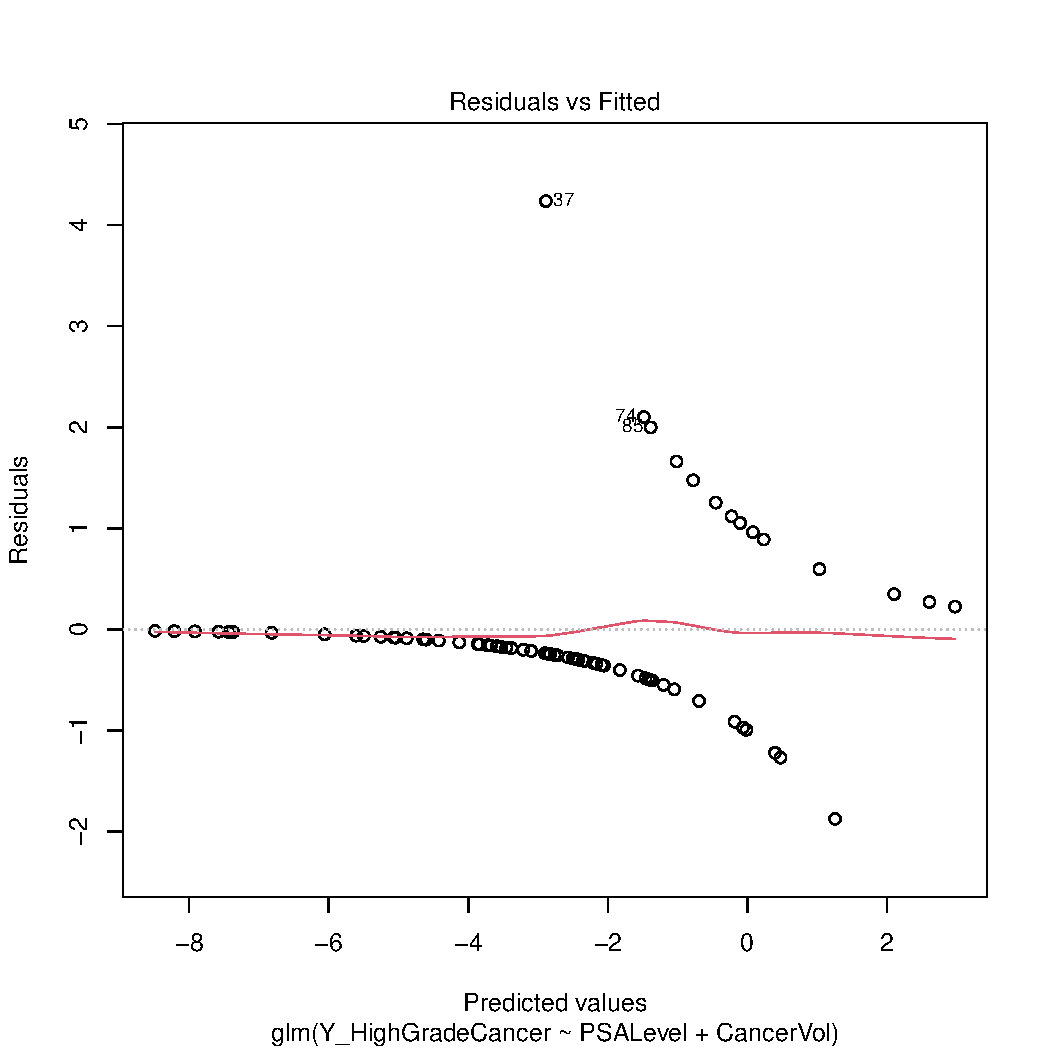
\includegraphics[width=\maxwidth]{figure/unnamed-chunk-1-2} 
\begin{kframe}\begin{alltt}
\hlcom{### build and plot ROC curve ###}
\hlstd{pred} \hlkwb{<-} \hlkwd{predict}\hlstd{(logit_red, train,} \hlkwc{type}\hlstd{=}\hlstr{"response"}\hlstd{)}
\hlstd{ROCRPred} \hlkwb{<-} \hlkwd{prediction}\hlstd{(pred, train}\hlopt{$}\hlstd{Y_HighGradeCancer)}
\hlstd{ROCRPref} \hlkwb{<-} \hlkwd{performance}\hlstd{(ROCRPred,} \hlstr{"tpr"}\hlstd{,} \hlstr{"fpr"}\hlstd{)}
\hlkwd{plot}\hlstd{(ROCRPref,} \hlkwc{colorize}\hlstd{=}\hlnum{TRUE}\hlstd{,} \hlkwc{print.cutoffs.at}\hlstd{=}\hlkwd{seq}\hlstd{(}\hlnum{0.1}\hlstd{,} \hlkwc{by}\hlstd{=}\hlnum{0.1}\hlstd{),}
     \hlkwc{main}\hlstd{=}\hlstr{"Reciever Operating Characteristic Curve"}\hlstd{)}
\end{alltt}
\end{kframe}
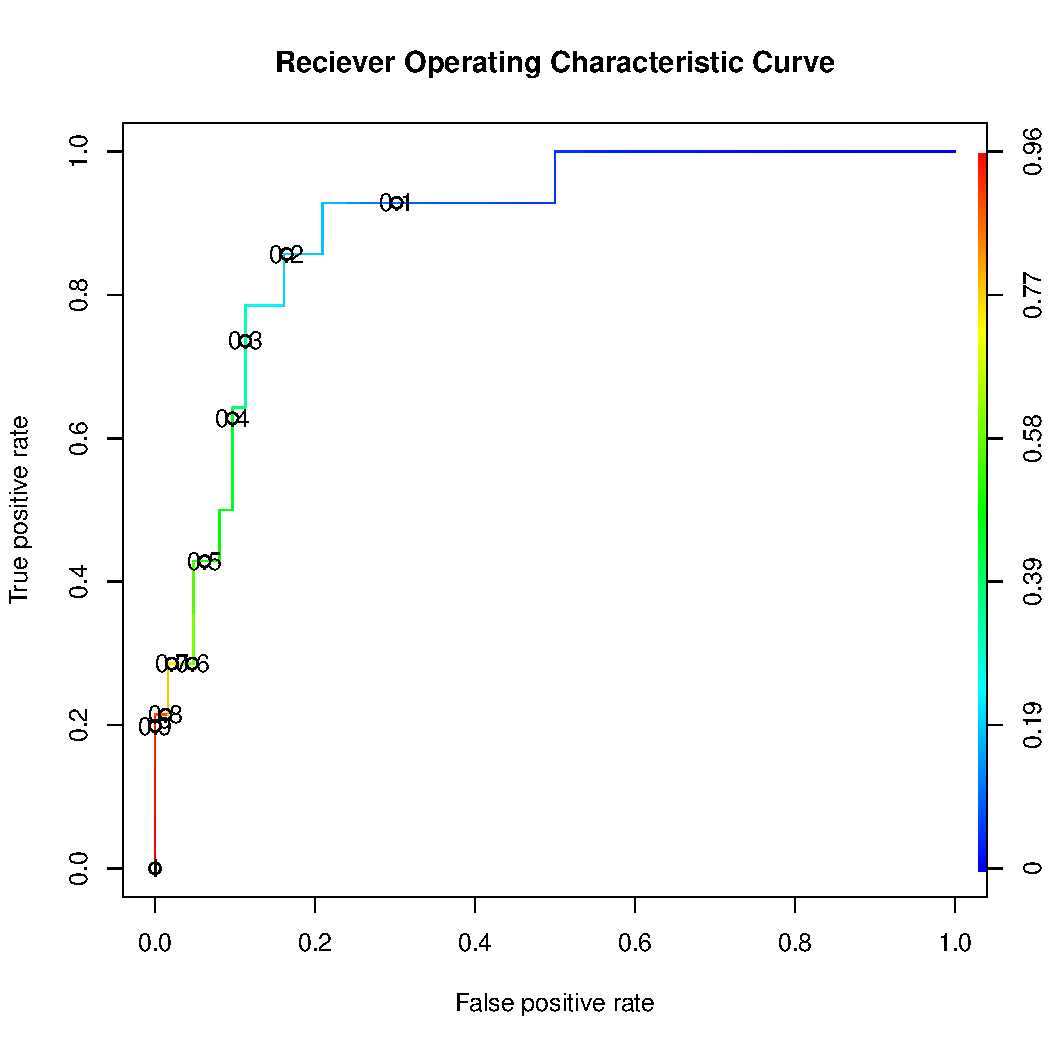
\includegraphics[width=\maxwidth]{figure/unnamed-chunk-1-3} 
\begin{kframe}\begin{alltt}
\hlcom{##################################}
\hlcom{### Accuracy Model Comparisons ###}
\hlcom{##################################}

\hlcom{### invoke functions ###}
\hlkwd{freq}\hlstd{(train)}
\end{alltt}
\begin{verbatim}
## TRAINING DATA
## Frequency Table:
## 
##  0  1 
## 62 14 
## 
## The proportion of 0 to 1 is: 0.8158 
## The proportion of 1 to 0 is: 0.1842
\end{verbatim}
\begin{alltt}
\hlkwd{accuracy}\hlstd{(logit_red, train,} \hlnum{0.184}\hlstd{)} \hlcom{# starting point prediction rule}
\end{alltt}
\begin{verbatim}
## TRAINING DATA
## Prediction Rule: 0.184 
## Confusion Matrix:
##  
##            PredictedValue
## ActualValue FALSE TRUE
##           0    49   13
##           1     1   13
## 
## The calculated error is: 18.4 %
## The calculated accuracy is: 81.6 %
\end{verbatim}
\begin{alltt}
\hlkwd{accuracy}\hlstd{(logit_red, train,} \hlnum{0.20}\hlstd{)} \hlcom{# final prediction rule}
\end{alltt}
\begin{verbatim}
## TRAINING DATA
## Prediction Rule: 0.2 
## Confusion Matrix:
##  
##            PredictedValue
## ActualValue FALSE TRUE
##           0    52   10
##           1     2   12
## 
## The calculated error is: 15.8 %
## The calculated accuracy is: 84.2 %
\end{verbatim}
\begin{alltt}
\hlcom{########################}
\hlcom{###                  ###}
\hlcom{###    Final Model   ###}
\hlcom{###                  ###}
\hlcom{########################}

\hlcom{# no changes have been made from the reduced model}
\hlstd{logit_final} \hlkwb{<-} \hlstd{logit_red}
\hlkwd{summary}\hlstd{(logit_final)}
\end{alltt}
\begin{verbatim}
## 
## Call:
## glm(formula = Y_HighGradeCancer ~ PSALevel + CancerVol, family = "binomial", 
##     data = train)
## 
## Deviance Residuals: 
##      Min        1Q    Median        3Q       Max  
## -1.73560  -0.43637  -0.23378  -0.03521   2.42555  
## 
## Coefficients:
##             Estimate Std. Error z value Pr(>|z|)    
## (Intercept)  -2.6867     0.6186  -4.343 1.41e-05 ***
## PSALevel      1.0577     0.6198   1.707   0.0879 .  
## CancerVol     1.5502     0.6859   2.260   0.0238 *  
## ---
## Signif. codes:  0 '***' 0.001 '**' 0.01 '*' 0.05 '.' 0.1 ' ' 1
## 
## (Dispersion parameter for binomial family taken to be 1)
## 
##     Null deviance: 72.613  on 75  degrees of freedom
## Residual deviance: 44.628  on 73  degrees of freedom
## AIC: 50.628
## 
## Number of Fisher Scoring iterations: 6
\end{verbatim}
\begin{alltt}
\hlcom{#########################################}
\hlcom{###                                   ###}
\hlcom{###    Model Validation: Test Data    ###}
\hlcom{###                                   ###}
\hlcom{#########################################}

\hlcom{##################################}
\hlcom{### Accuracy Model Comparisons ###}
\hlcom{##################################}

\hlcom{### invoke functions ###}
\hlkwd{freq}\hlstd{(test)}
\end{alltt}
\begin{verbatim}
## TESTING DATA
## Frequency Table:
## 
##  0  1 
## 14  7 
## 
## The proportion of 0 to 1 is: 0.6667 
## The proportion of 1 to 0 is: 0.3333
\end{verbatim}
\begin{alltt}
\hlkwd{accuracy}\hlstd{(logit_final, test,} \hlnum{0.20}\hlstd{)}
\end{alltt}
\begin{verbatim}
## TESTING DATA
## Prediction Rule: 0.2 
## Confusion Matrix:
##  
##            PredictedValue
## ActualValue FALSE TRUE
##           0    13    1
##           1     2    5
## 
## The calculated error is: 14.3 %
## The calculated accuracy is: 85.7 %
\end{verbatim}
\end{kframe}
\end{knitrout}

\end{document}
